\documentclass[12pt, fullpage,letterpaper]{article}

\usepackage[margin=1in]{geometry}
\usepackage{url}
\usepackage{amsmath}
\usepackage{amssymb}
\usepackage{xspace}
\usepackage{graphicx}
\usepackage{hyperref}
\usepackage{listings}

\newcommand{\semester}{Fall 2021}
\newcommand{\assignmentId}{3}
\newcommand{\releaseDate}{19 Oct, 2021}
\newcommand{\dueDate}{11:59pm, 2 Nov, 2021}

\newcommand{\bx}{{\bf x}}
\newcommand{\bw}{{\bf w}}

\title{CS 5350/6350: Machine Learining \semester}
\author{Homework \assignmentId}
\date{Handed out: \releaseDate\\
	Due: \dueDate}


\title{CS 5350/6350: Machine Learning \semester}
\author{Homework \assignmentId}
\date{Handed out: \releaseDate\\
  Due date: \dueDate}

\begin{document}
\maketitle

% Math commands by Thomas Minka
\newcommand{\var}{{\rm var}}
\newcommand{\Tr}{^{\rm T}}
\newcommand{\vtrans}[2]{{#1}^{(#2)}}
\newcommand{\kron}{\otimes}
\newcommand{\schur}[2]{({#1} | {#2})}
\newcommand{\schurdet}[2]{\left| ({#1} | {#2}) \right|}
\newcommand{\had}{\circ}
\newcommand{\diag}{{\rm diag}}
\newcommand{\invdiag}{\diag^{-1}}
\newcommand{\rank}{{\rm rank}}
% careful: ``null'' is already a latex command
\newcommand{\nullsp}{{\rm null}}
\newcommand{\tr}{{\rm tr}}
\renewcommand{\vec}{{\rm vec}}
\newcommand{\vech}{{\rm vech}}
\renewcommand{\det}[1]{\left| #1 \right|}
\newcommand{\pdet}[1]{\left| #1 \right|_{+}}
\newcommand{\pinv}[1]{#1^{+}}
\newcommand{\erf}{{\rm erf}}
\newcommand{\hypergeom}[2]{{}_{#1}F_{#2}}

% boldface characters
\renewcommand{\a}{{\bf a}}
\renewcommand{\b}{{\bf b}}
\renewcommand{\c}{{\bf c}}
\renewcommand{\d}{{\rm d}}  % for derivatives
\newcommand{\e}{{\bf e}}
\newcommand{\f}{{\bf f}}
\newcommand{\g}{{\bf g}}
\newcommand{\h}{{\bf h}}
%\newcommand{\k}{{\bf k}}
% in Latex2e this must be renewcommand
\renewcommand{\k}{{\bf k}}
\newcommand{\m}{{\bf m}}
\newcommand{\mb}{{\bf m}}
\newcommand{\n}{{\bf n}}
\renewcommand{\o}{{\bf o}}
\newcommand{\p}{{\bf p}}
\newcommand{\q}{{\bf q}}
\renewcommand{\r}{{\bf r}}
\newcommand{\s}{{\bf s}}
\renewcommand{\t}{{\bf t}}
\renewcommand{\u}{{\bf u}}
\renewcommand{\v}{{\bf v}}
\newcommand{\w}{{\bf w}}
\newcommand{\x}{{\bf x}}
\newcommand{\y}{{\bf y}}
\newcommand{\z}{{\bf z}}
%s\newcommand{\l}{\boldsymbol{l}}
\newcommand{\A}{{\bf A}}
\newcommand{\B}{{\bf B}}
\newcommand{\C}{{\bf C}}
\newcommand{\D}{{\bf D}}
\newcommand{\E}{{\bf E}}
\newcommand{\F}{{\bf F}}
\newcommand{\G}{{\bf G}}
\renewcommand{\H}{{\bf H}}
\newcommand{\I}{{\bf I}}
\newcommand{\J}{{\bf J}}
\newcommand{\K}{{\bf K}}
\renewcommand{\L}{{\bf L}}
\newcommand{\M}{{\bf M}}
\newcommand{\N}{\mathcal{N}}  % for normal density
%\newcommand{\N}{{\bf N}}
\renewcommand{\O}{{\bf O}}
\renewcommand{\P}{{\bf P}}
\newcommand{\Q}{{\bf Q}}
\newcommand{\R}{{\bf R}}
\renewcommand{\S}{{\bf S}}
\newcommand{\T}{{\bf T}}
\newcommand{\U}{{\bf U}}
\newcommand{\V}{{\bf V}}
\newcommand{\W}{{\bf W}}
\newcommand{\X}{{\bf X}}
\newcommand{\Y}{{\bf Y}}
\newcommand{\Z}{{\bf Z}}

% this is for latex 2.09
% unfortunately, the result is slanted - use Latex2e instead
%\newcommand{\bfLambda}{\mbox{\boldmath$\Lambda$}}
% this is for Latex2e
\newcommand{\bfLambda}{\boldsymbol{\Lambda}}

% Yuan Qi's boldsymbol
\newcommand{\bsigma}{\boldsymbol{\sigma}}
\newcommand{\balpha}{\boldsymbol{\alpha}}
\newcommand{\bpsi}{\boldsymbol{\psi}}
\newcommand{\bphi}{\boldsymbol{\phi}}
\newcommand{\boldeta}{\boldsymbol{\eta}}
\newcommand{\Beta}{\boldsymbol{\eta}}
\newcommand{\btau}{\boldsymbol{\tau}}
\newcommand{\bvarphi}{\boldsymbol{\varphi}}
\newcommand{\bzeta}{\boldsymbol{\zeta}}

\newcommand{\blambda}{\boldsymbol{\lambda}}
\newcommand{\bLambda}{\mathbf{\Lambda}}
\newcommand{\bOmega}{\mathbf{\Omega}}
\newcommand{\bomega}{\mathbf{\omega}}
\newcommand{\bPi}{\mathbf{\Pi}}

\newcommand{\btheta}{\boldsymbol{\theta}}
\newcommand{\bpi}{\boldsymbol{\pi}}
\newcommand{\bxi}{\boldsymbol{\xi}}
\newcommand{\bSigma}{\boldsymbol{\Sigma}}

\newcommand{\bgamma}{\boldsymbol{\gamma}}
\newcommand{\bGamma}{\mathbf{\Gamma}}

\newcommand{\bmu}{\boldsymbol{\mu}}
\newcommand{\1}{{\bf 1}}
\newcommand{\0}{{\bf 0}}

% \newcommand{\comment}[1]{}

\newcommand{\bs}{\backslash}
\newcommand{\ben}{\begin{enumerate}}
\newcommand{\een}{\end{enumerate}}

 \newcommand{\notS}{{\backslash S}}
 \newcommand{\nots}{{\backslash s}}
 \newcommand{\noti}{{\backslash i}}
 \newcommand{\notj}{{\backslash j}}
 \newcommand{\nott}{\backslash t}
 \newcommand{\notone}{{\backslash 1}}
 \newcommand{\nottp}{\backslash t+1}
% \newcommand{\notz}{\backslash z}

\newcommand{\notk}{{^{\backslash k}}}
%\newcommand{\noti}{{^{\backslash i}}}
\newcommand{\notij}{{^{\backslash i,j}}}
\newcommand{\notg}{{^{\backslash g}}}
\newcommand{\wnoti}{{_{\w}^{\backslash i}}}
\newcommand{\wnotg}{{_{\w}^{\backslash g}}}
\newcommand{\vnotij}{{_{\v}^{\backslash i,j}}}
\newcommand{\vnotg}{{_{\v}^{\backslash g}}}
\newcommand{\half}{\frac{1}{2}}
\newcommand{\msgb}{m_{t \leftarrow t+1}}
\newcommand{\msgf}{m_{t \rightarrow t+1}}
\newcommand{\msgfp}{m_{t-1 \rightarrow t}}

\newcommand{\proj}[1]{{\rm proj}\negmedspace\left[#1\right]}
\newcommand{\argmin}{\operatornamewithlimits{argmin}}
\newcommand{\argmax}{\operatornamewithlimits{argmax}}

\newcommand{\dif}{\mathrm{d}}
\newcommand{\abs}[1]{\lvert#1\rvert}
\newcommand{\norm}[1]{\lVert#1\rVert}

%miscellaneous symbols
\newcommand{\ie}{{{i.e.,}}\xspace}
\newcommand{\eg}{{{\em e.g.,}}\xspace}
\newcommand{\EE}{\mathbb{E}}
\newcommand{\VV}{\mathbb{V}}
\newcommand{\sbr}[1]{\left[#1\right]}
\newcommand{\rbr}[1]{\left(#1\right)}
\newcommand{\cmt}[1]{}


\newcommand{\Hcal}{\mathcal{H}} 
{\footnotesize
	\begin{itemize}
		\item You are welcome to talk to other members of the class about
		the homework. I am more concerned that you understand the
		underlying concepts. However, you should write down your own
		solution. Please keep the class collaboration policy in mind.
		
		\item Feel free to discuss the homework with the instructor or the TAs.
		
		\item Your written solutions should be brief and clear. You do not need to include original problem descriptions in your solutions. You need to
		show your work, not just the final answer, but you do \emph{not}
		need to write it in gory detail. Your assignment should be {\bf no
			more than 15 pages}. Every extra page will cost a point.
		
		\item Handwritten solutions will not be accepted.
		
		
		\item {\em Your code should run on the CADE machines}. \textbf{You should
		include a shell script, {\tt run.sh}, that will execute your code
		in the CADE environment. Your code should produce similar output to what you include in your report.}
		
		You are responsible for ensuring that the grader can execute the
		code using only the included script. If you are using an
		esoteric programming language, you should make sure that its
		runtime is available on CADE.
		
		\item Please do not hand in binary files! We will {\em not} grade
		binary submissions.
		
		\item The homework is due by \textbf{midnight of the due date}. Please submit
		the homework on Canvas.
		
	\end{itemize}
}


\section{Paper Problems [36 points + 15 bonus]}
\begin{enumerate}
	\item~[8 points] Suppose we have a linear classifier for $2$ dimensional features. The classification boundary, \ie  the hyperplane is $2x_1 + 3x_2 - 4 = 0$ ($x_1$ and $x_2$ are the two input features). 
	
	$dist(\x_i, h) = \frac{|\w^\top \x_i + b|}{||\w||}$
	
	\begin{enumerate}
	
	\begin{table}[h]
		\centering
		\begin{tabular}{cc|c||c}
			$x_1$ & $x_2$ &  {label} & {distance}\\ 
			\hline\hline
			1  &  1 &  1 & $\frac{1}{\sqrt{13}} | 2 *  1 + 3 * 1 - 4 | = \frac{1}{\sqrt{13}}$ \\ \hline
			1  & -1 & -1 & $\frac{1}{\sqrt{13}} | 2 *  1 - 3 * 1 - 4 | = \frac{5}{\sqrt{13}}$ \\ \hline
			0  &  0 & -1 & $\frac{1}{\sqrt{13}} | 2 *  0 + 3 * 0 - 4 | = \frac{4}{\sqrt{13}}$ \\ \hline
			-1 & 3  &  1 & $\frac{1}{\sqrt{13}} | 2 * -1 + 3 * 3 - 4 | = \frac{3}{\sqrt{13}}$ \\ \hline
			\end{tabular}
		\caption{Dataset 1, with distance calculations}
	\end{table}
	\item~[4 points] Now we have a dataset in Table 1. 
	Does the hyperplane have a margin for the dataset?  If yes, what is the margin? Please use the formula we discussed in the class to compute. If no, why? (Hint: when can a hyperplane have a margin?)
	
	\begin{table}[h]
		\centering
		\begin{tabular}{cc|c}
			$x_1$ & $x_2$ &  {label}\\ 
			\hline\hline
			1  &  1 &  1 \\ \hline
			1  & -1 & -1 \\ \hline
			0  &  0 & -1 \\ \hline
			-1 &  3 &  1 \\ \hline
		    -1 & -1 &  1 \\
		\end{tabular}
		\caption{Dataset 2}
	\end{table}
	
	\emph{Answer}
	
	Figure 1 demonstrates that this hyperplane does separate the data. Table 1 (updated with Distance calculations) gives the distance between each data point and the hyperplane. The minimum distance is $\frac{1}{\sqrt{13}}$, which means that is the margin.
	
	\begin{figure}[htp]
        \centering
        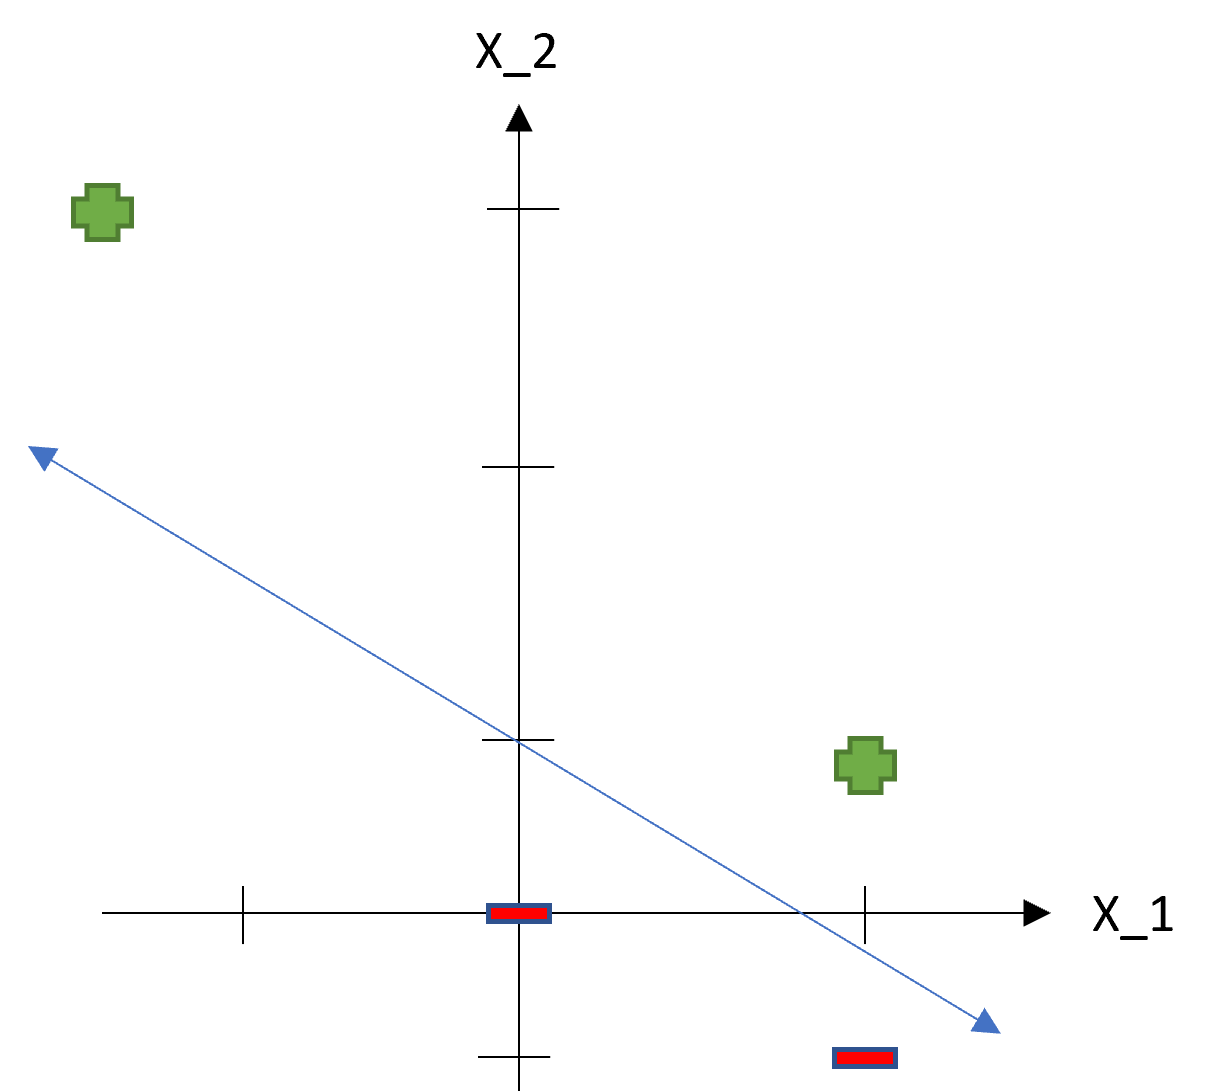
\includegraphics[width=8cm]{part1_q1a.png}
        \caption{Weight vector change per update.}
        \label{fig:q2b_weights}
    \end{figure}
	
	\item~[4 points] We have a second dataset in Table 2. Does the hyperplane have a margin for the dataset? If yes, what is the margin? If no, why? 
	
	\emph{Answer}
	
	Figure 2 plots the hyperplane and the data points. Clearly, the hyperplane does not separate the data correctly, so there can be no margin.
	
	\begin{figure}[htp]
        \centering
        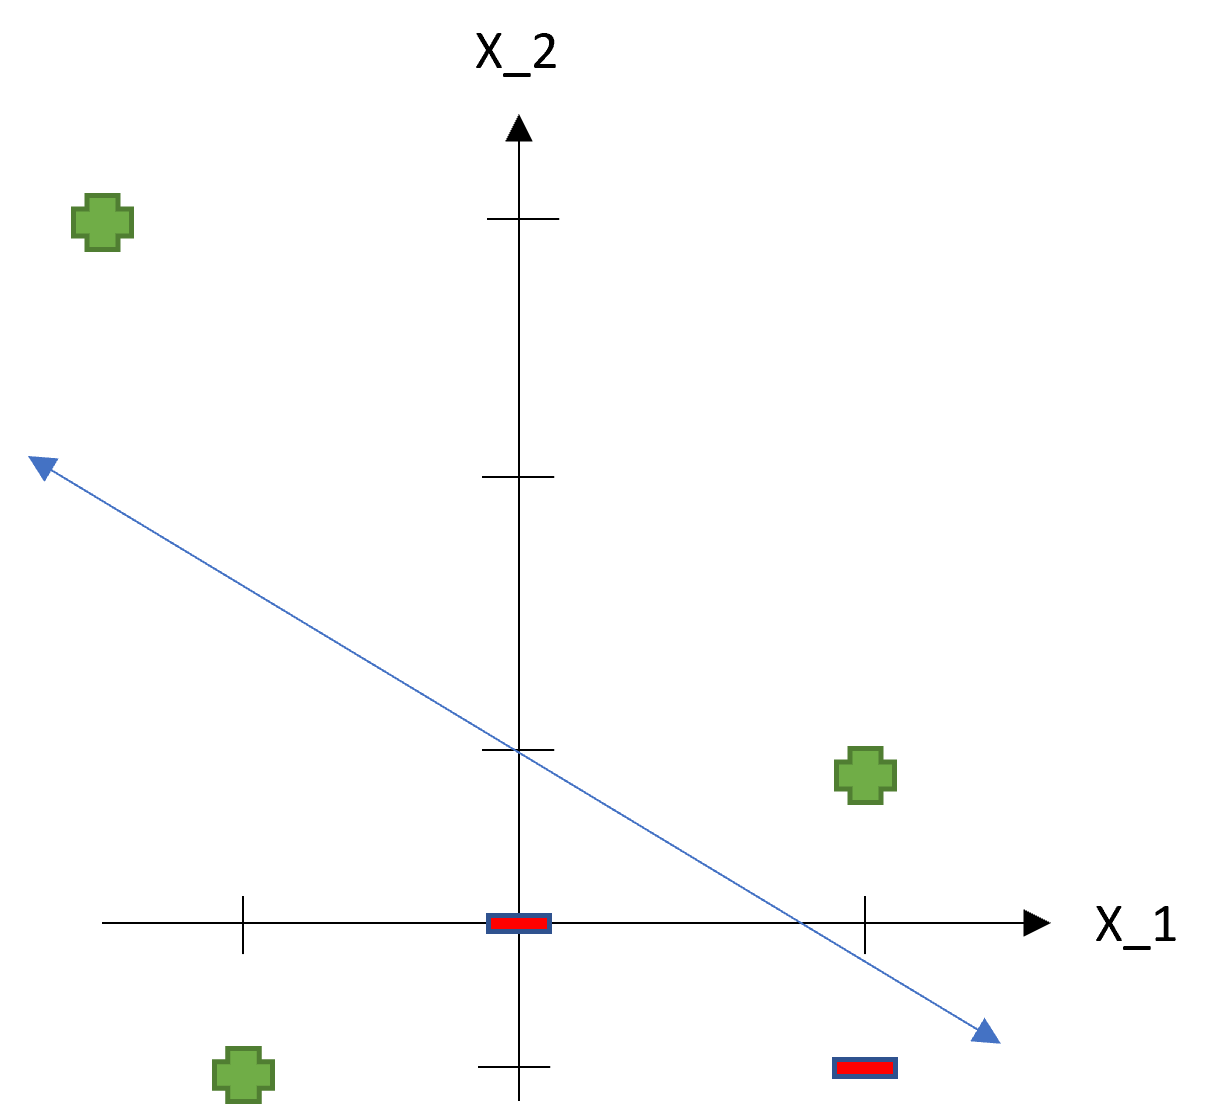
\includegraphics[width=8cm]{part1_q1b.png}
        \caption{Weight vector change per update.}
        \label{fig:q2b_weights}
    \end{figure}
	
	\end{enumerate}
	

		\item~[8 points] Now, let us look at margins for datasets. Please review what we have discussed in the lecture and slides. A margin for a dataset is not a margin of a hyperplane!  
		
		
		\begin{enumerate}
			
			\begin{table}[h]
				\centering
				\begin{tabular}{cc|c|c}
					$x_1$ & $x_2$ &  {label} & {distance} \\ 
					\hline\hline
					-1 &  0 & -1 & $\frac{1}{\sqrt{2}} | -1 + 0 | = \frac{1}{\sqrt{2}}$ \\ \hline
					 0 & -1 & -1 & $\frac{1}{\sqrt{2}} |  0 - 1 | = \frac{1}{\sqrt{2}}$ \\ \hline
					 1 &  0 &  1 & $\frac{1}{\sqrt{2}} |  1 + 0 | = \frac{1}{\sqrt{2}}$ \\ \hline
					 0 &  1 &  1 & $\frac{1}{\sqrt{2}} |  0 + 1 | = \frac{1}{\sqrt{2}}$ \\ \hline
				\end{tabular}
				\caption{Dataset 3, with distance calculations}
			\end{table}
			
			\item~[4 points] Given the dataset in Table 3, can you calculate its margin? If you cannot, please explain why. 
			
			\emph{Answer}
		
    		Figure 3 plots Dataset 3 and a potential hyperplane that would separate the data. We can calculate R, which is the furthest point from the origin, but all points are equidistant from the origin, so they all have the same R. We see that $R = \sqrt{0^2 + 1^2} = 1$. If we use a simple hyperplane that goes through the origin and has the same distance to all four points, say $x_1 + x_2 = 0$, we see that $||\w|| = \sqrt{1^2 + 1^2} = \sqrt{2}$
    		
    		\begin{figure}[htp]
                \centering
                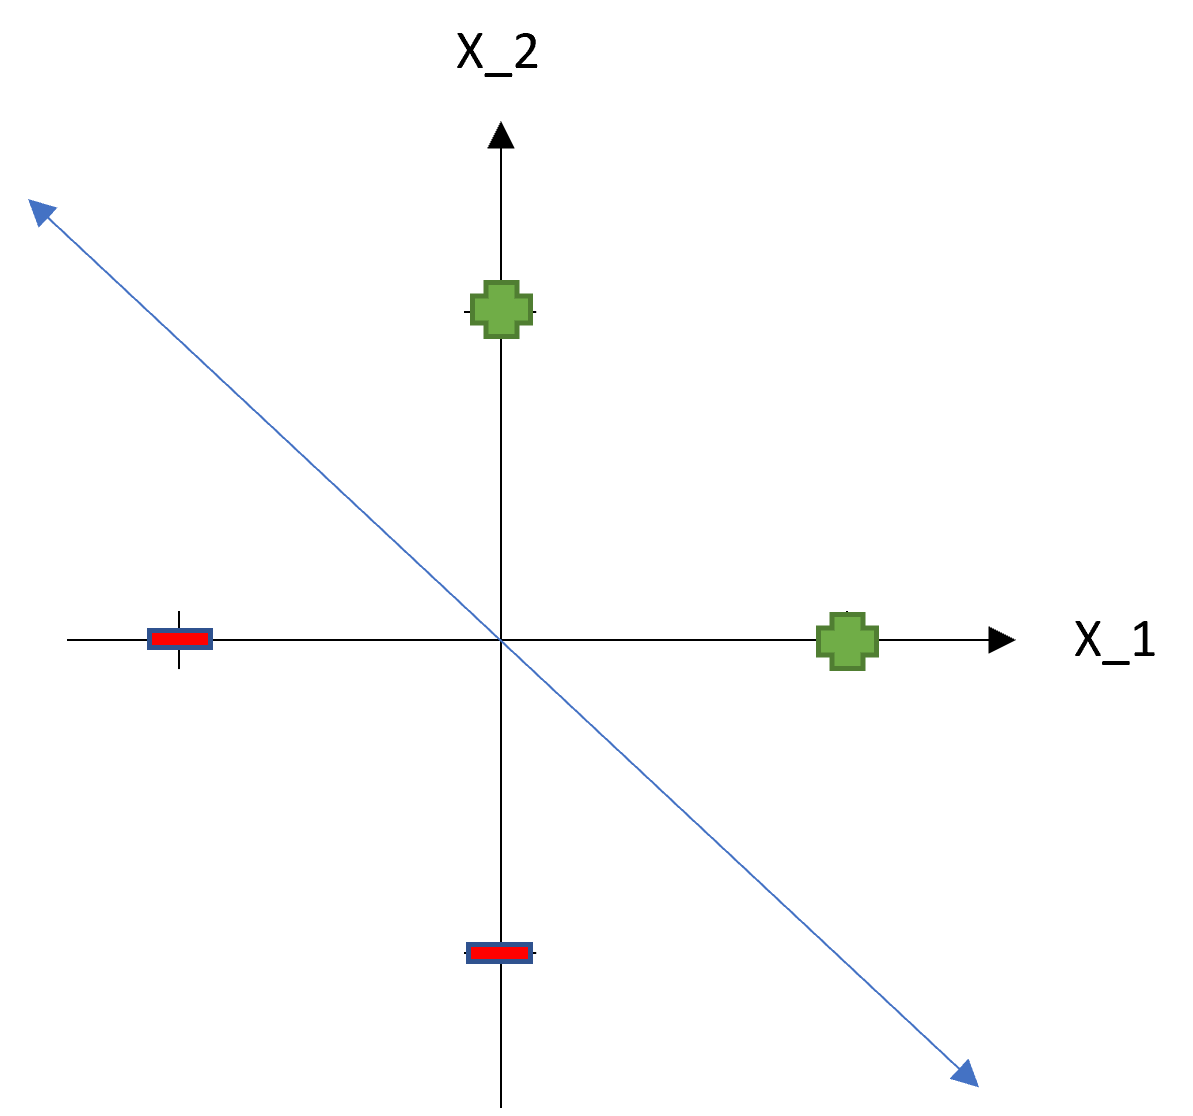
\includegraphics[width=8cm]{part1_q2a.png}
                \caption{Weight vector change per update.}
                \label{fig:q2b_weights}
            \end{figure}
			
			\begin{table}[h]
				\centering
				\begin{tabular}{cc|c}
					$x_1$ & $x_2$ &  {label}\\ 
					\hline\hline
						-1 & 0 & -1 \\ \hline
					0 & -1 & 1 \\ \hline
					1 & 0 & -1 \\ \hline
					0 & 1 & 1 \\ \hline
				\end{tabular}
				\caption{Dataset 4}
			\end{table}
			
			\item~[4 points] Given the dataset in Table 4, can you calculate its margin? If you cannot, please explain why. 
			
			\emph{Answer}
			
			Figure 4 plots Dataset 4. Clearly, the data is not linearly separable, so we cannot calculate any margin.
			
			\begin{figure}[htp]
                \centering
                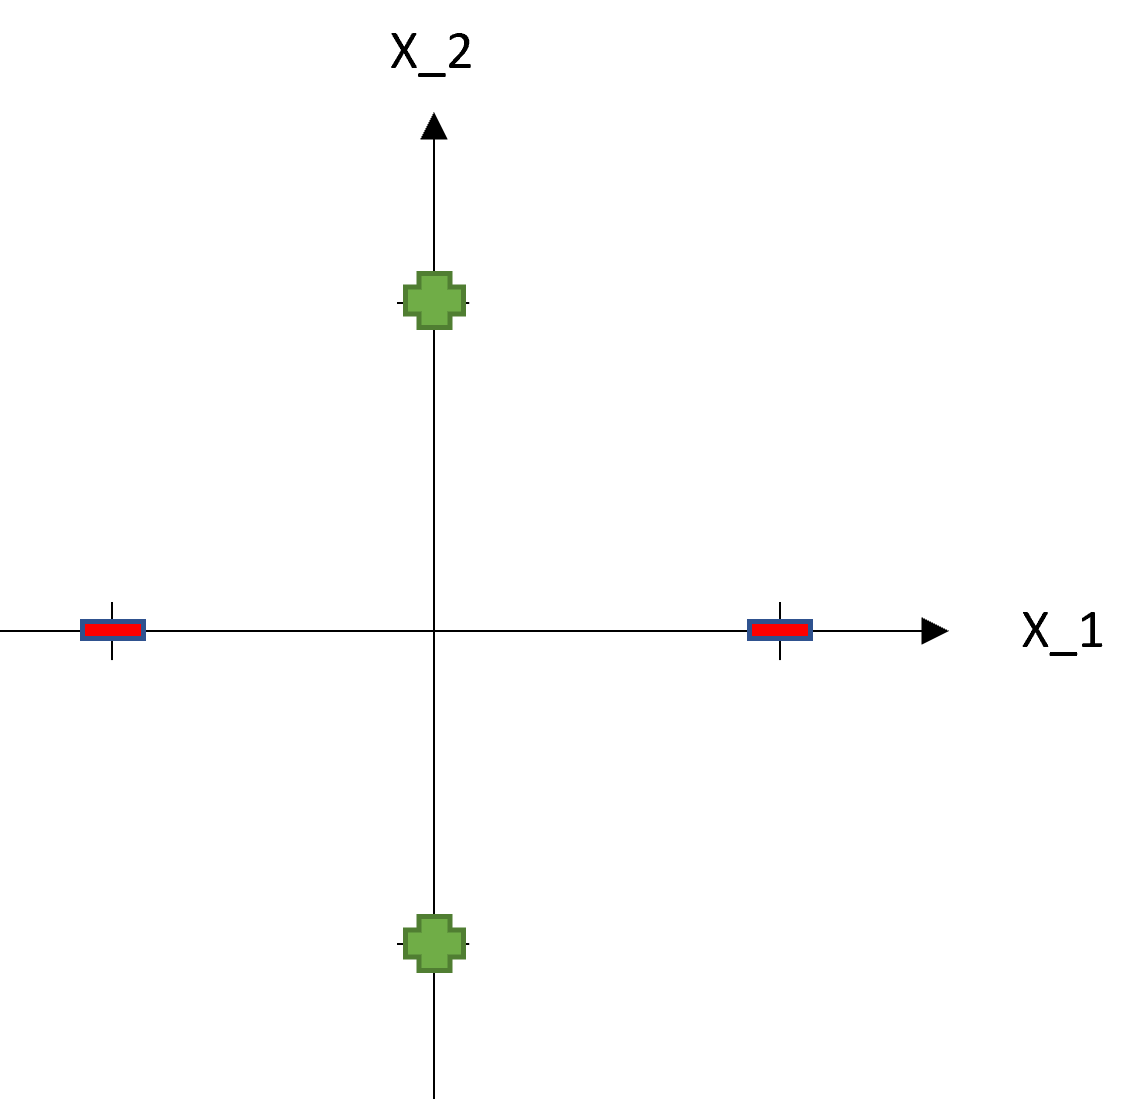
\includegraphics[width=8cm]{part1_q2b.png}
                \caption{Weight vector change per update.}
                \label{fig:q2b_weights}
            \end{figure}
			
		\end{enumerate}
	
	\item ~[\textbf{Bonus}] [5 points] Let us review the Mistake Bound Theorem for Perceptron discussed in our lecture.  If we change the second assumption to be as follows: Suppose there exists a vector $\u\in \mathbb{R}^n$, and a positive $\gamma$, we have for each $(\x_i, y_i)$ in the training data, $y_i(\u^\top \x_i) \ge \gamma$. What is the upper bound for the number of mistakes made by the Perceptron algorithm?   Note that $\u$ is unnecessary to be a unit vector.
	
	\emph{Answer}
	
	Comparing to the proof in the lecture slides \href{https://www.cs.utah.edu/~zhe/teach/pdf/Perceptron.pdf}{(CLICK HERE)}, the only difference is that $\u$ is not \emph{necessarily} a unit vector. We will note that normally, the upper bound is $\frac{R^2}{\gamma^2}$.
	
	We will pick up at part 3/3 of the proof seen in the lecture slides. We know that $\u^\top \w_t \geq t \gamma$ and $t R^2 \geq ||\w_t||^2$, the latter of which can be rewritten as $\sqrt{t} R \geq ||\w_t||$. We can also rewrite the dot product $\u^\top \w$ as $||\u|| ||\w_t|| cos\theta$, where $\theta$ is the angle between $\u$ and $\w_t$, and $cos\theta < 1$. The interesting case for us is when $||\u|| ||\w_t|| cos\theta > ||\w_t||$, which means that $||\u|| > \frac{1}{cos\theta}$. 
	
	Obviously, based on Proof 3/3 from the lecture slides, if $||\u|| \leq \frac{1}{cos\theta}$, then we get $\frac{R^2}{\gamma^2}$.
	
	If $||\u|| > \frac{1}{cos\theta}$,
	
	\[
	    => ||\u|| ||\w_t|| cos\theta \geq t\gamma
	\]
	\[
	    => ||\w_t|| \geq \frac{t\gamma}{||\u|| cos\theta}
	\]
	
	From here, we add in that $\sqrt{t} R \geq ||\w_t||$ to yield,
	
	\[
	    R \sqrt{t} \geq ||\w_t|| \geq \frac{t\gamma}{||\u|| cos\theta}
	\]
	\[
	    => R^2 t \geq \frac{t^2 \gamma^2}{||\u||^2 cos^2\theta}
	\]
	\[
	    => ||\u||^2 cos^2\theta \frac{R^2}{\gamma^2} \geq t
	\]
	
	So, it is the same value as the upper bound for when $\u$ is a unit vector, but scaled by the square of the norm of $\u$ and the cosine of its angle with $\w_t$. Obviously, this means it is simpler to compute the upper bound if we just keep $\u$ as a unit vector.
	
	\begin{figure}[htp]
        \centering
        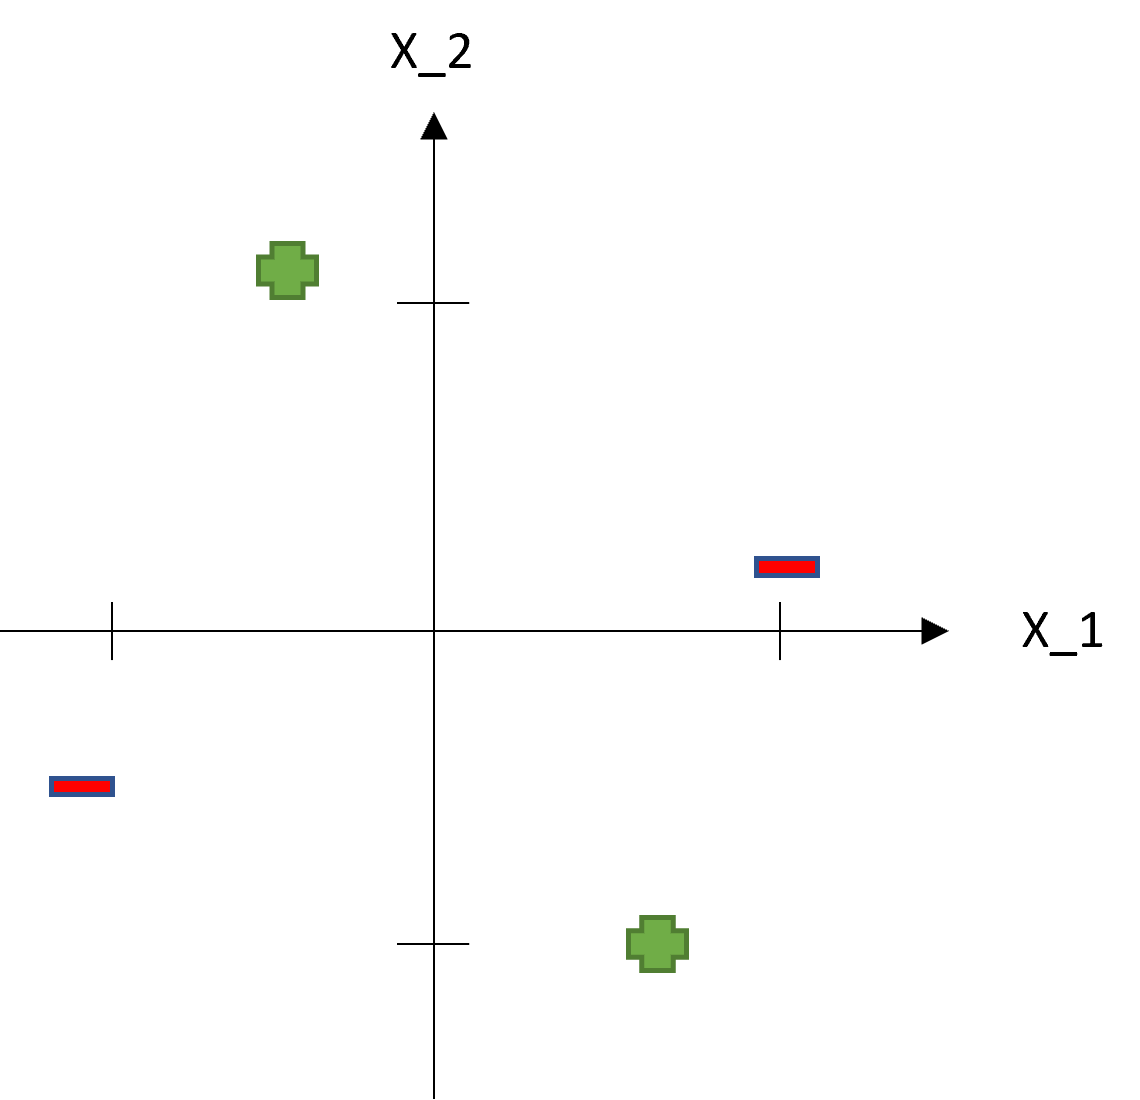
\includegraphics[width=8cm]{part1_q5.png}
        \caption{Weight vector change per update.}
        \label{fig:q2b_weights}
    \end{figure}
	
	\item~[10 points] We want to use Perceptron to learn a disjunction as follows,
	\[
	f(x_1, x_2, \ldots, x_n) = \neg x_1 \lor \neg \ldots \neg x_k \lor x_{k+1} \lor \ldots \lor x_{2k} \;\;\;\;(\mathrm{note\; that}\;\; 2k < n).
	\]
	The training set are all $2^n$ Boolean input vectors in the instance space. 
	Please derive an upper bound of the number of mistakes made by Perceptron in learning this disjunction.

	\item~[10 points] Prove that linear classifiers in a plane cannot shatter any $4$ distinct points. 
	
	\emph{Answer}
	
	Figure 5 shows a case with four points that cannot be shattered by any linear classifier.
	
	\item~[\textbf{Bonus}]~[10 points] Consider our infinite hypothesis space $\Hcal$ are all rectangles in a plain. Each rectangle corresponds to a classifier --- all the points inside the rectangle are classified as positive, and otherwise classified as negative. What is $\mathrm{VC}(\Hcal)$? 


\end{enumerate}

\section{Practice [64 points ]}
\begin{enumerate}
	\item~[2 Points] Update your machine learning library. Please check in your implementation of ensemble learning and least-mean-square (LMS) method in HW1 to your GitHub repository. Remember last time you created the folders ``Ensemble Learning" and ``Linear Regression''. You can commit your code into the corresponding folders now. Please also supplement README.md with concise descriptions about how to use your code to run your Adaboost, bagging, random forest, LMS with batch-gradient and stochastic gradient (how to call the command, set the parameters, etc). Please create a new folder ``Perceptron" in the same level as these folders.
	
	\href{https://github.com/Paul-Wissler/cs-6350-hw3}{Click here for the repository for HW3}. It is not the same as the repository for HW1 or HW2.

\item We will implement  Perceptron for a binary classification task --- bank-note authentication. Please download the data ``bank-note.zip'' from Canvas. The features and labels are listed in the file ``bank-note/data-desc.txt''. The training data are stored in the file ``bank-note/train.csv'', consisting of $872$ examples. The test data are stored in ``bank-note/test.csv'', and comprise of $500$ examples. In both the training and testing datasets, feature values and labels are separated by commas. 
\begin{enumerate}
	\item~[16 points] Implement the standard Perceptron. Set the maximum number of epochs $T$ to 10. Report your learned weight vector, and the average prediction error on the test dataset. 
	
	\emph{Answer}
	
	WEIGHT VECTOR
	
	WaveletVariance   -5.777450
	
    WaveletSkew       -3.204904
    
    WaveletCurtosis   -4.753204
    
    ImageEntropy      -0.603608
    
    MODEL\_BIAS        -5.300000
    
    ERRORS
	
	TRAIN ERROR:  0.04243
	
    TEST ERROR:   0.05000
	
	\item~[16 points] Implement the voted Perceptron. Set the maximum number of epochs $T$ to 10. Report the list of the distinct weight vectors and their counts --- the number of correctly predicted training examples. Using this set of weight vectors to predict each test example. Report the average test error. 
	
	\emph{Answer}
	
	Figure 6 shows how the weight vector changes with each update, and Figure 7 shows the votes assigned to each weight vector. The votes correspond to how many data points that each weight vector managed to accurately predict.
	
	\begin{figure}[htp]
        \centering
        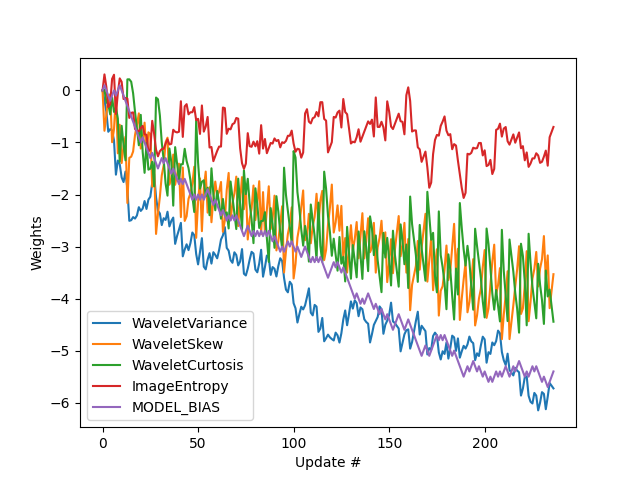
\includegraphics[width=12cm]{q2b_weights_convergence.png}
        \caption{Weight vector change per update.}
        \label{fig:q2b_weights}
    \end{figure}
    
    \begin{figure}[htp]
        \centering
        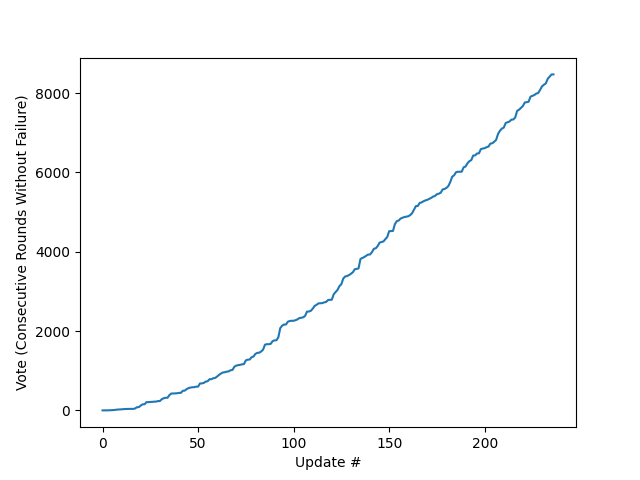
\includegraphics[width=12cm]{q2b_votes.png}
        \caption{Votes for each weight vector.}
        \label{fig:q2b_votes}
    \end{figure}
	
	TRAIN ERROR:  0.01261
	
    TEST ERROR:   0.01400
	
	\item~[16 points] Implement the average Perceptron. Set the maximum number of epochs $T$ to 10. Report your learned weight vector. Comparing with the list of weight vectors from (b), what can you observe? Report the average prediction error on the test data. 
	
	\emph{Answer}
	
	WEIGHT VECTOR
	WaveletVariance   -37108.434439
	
    WaveletSkew       -25185.487162
    
    WaveletCurtosis   -25383.376175
    
    ImageEntropy       -7638.087261
    
    MODEL\_BIAS        -34243.400000
    
    ERRORS
	
	TRAIN ERROR:  0.01491
    
    TEST ERROR:   0.01400
	
	\item~[14 points] Compare the average prediction errors for the three methods. What do you conclude? 
	
	Obviously, the standard Perceptron is the worst performer. But, Voted and Average Perceptrons perform about the same. Because the Voted Perceptron stores more data, the Average Perceptron is likely a more performative model at higher epochs since it only needs to compare to evaluate with one weight vector.
	
\end{enumerate}


\end{enumerate}

\end{document}
%%% Local Variables:
%%% mode: latex
%%% TeX-master: t
%%% End:
